\documentclass[11pt]{amsart}


\usepackage{geometry}                % See geometry.pdf to learn the layout options. There are lots.
\geometry{a4paper}                   % ... or a4paper or a5paper or ...
%\geometry{landscape}                % Activate for for rotated page geometry
\usepackage[parfill]{parskip}    % Activate to begin paragraphs with an empty line rather than an indent
\usepackage{enumitem}
\usepackage{graphicx}
\usepackage{amssymb}
\usepackage{amsmath}
\usepackage{cancel}
\usepackage{epstopdf}
\DeclareGraphicsRule{.tif}{png}{.png}{`convert #1 `dirname #1`/`basename #1 .tif`.png}
\usepackage{breqn}
\usepackage{float}

\title{Econ 220C Problem Set \# 2}
\author{Minki Kim}
%\date{}                                           % Activate to display a given date or no date

\begin{document}




\maketitle

\section{Investment and the Housing Market}
\subsection{Explain the model}
\begin{enumerate}
	\item $I = \psi (P)$: Gross investment in housing is an increasing function of the price of houses. This specification makes sense because housing investment is interpreted as housing supply. 
	\item $r + \delta = (R + \dot{P})/P$: I assume that $\delta$ denotes the depreciation rate of a house. LHS is opportunity costs of owning a house: forgone rental interest rate and depreciation of the house. RHS is benefits of owning a house: (real) rental payment and capital gains. 
	\item $R = R(H)$: Rental cost $R$ is a decreasing function of available quantity of housing stock. 
	\item $\dot{H} = I - \delta H$: Change in $H$ is the difference between housing investment (new housing) and depreciated housing stock. 
\end{enumerate}
The model is closed: it has 4 endogenous variables ($I,R,P,H$) with 4 equations.

\subsection{Reduce the model into a 2-equation system}
\begin{align*}
\dot{H} &= \psi(P) - \delta H \\
r + \delta &= (R(H) + \dot{P}) / P
\end{align*}
Here $R$ is a function, not a variable. 
\subsection{Draw phase diagram}
*Lines do not have to be linear. 
\begin{figure}[H]
	\centering
	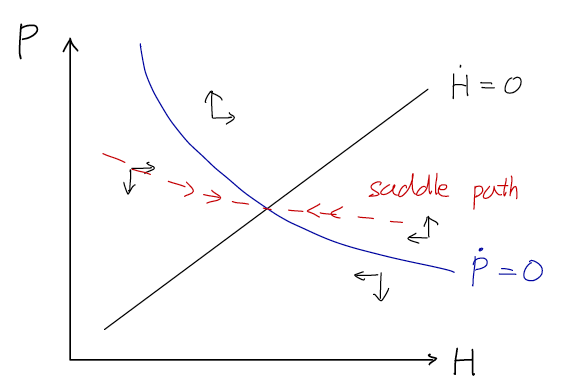
\includegraphics[width=0.55\textwidth]{1c_Minki.png}
\end{figure}

\subsection{Steady state effect of $r$}

\section{Discount Factor Shock}
\section{News Shock}
\section{Labor Supply}
\section{Impulse Responses}
\section{Impulse Responses (2)}



\end{document}
